% !TEX program = xelatex
\documentclass[a4paper,12pt, oneside]{article}
\usepackage[utf8]{inputenc}

\usepackage{graphicx} % To include images
%\usepackage{color} % To have more colors and be able to define new one
\usepackage{xcolor} % To have more colors and be able to define new one
\usepackage{afterpage} % For the page background color
\usepackage{listings} % To include code snippets
\usepackage{indentfirst} % To indent the first paragraph
\usepackage{url} % For url...
\usepackage[all]{nowidow} % To prevent widow/orphan lines
\usepackage[margin=2.5cm]{geometry} % To change the margin
\usepackage[justification=justified,singlelinecheck=false]{caption} % To left align even the single line captions
\usepackage{multicol} % Enable multi columns environment
\usepackage{subcaption} % To have two figures next to each other
\usepackage{fontspec} % For custom fonts
\usepackage{lipsum} % Lorem ipsum generator
\usepackage{layouts} %to get the text width in cm
\usepackage{rotating} %to have some figures sideways.

\usepackage{tikz}
\usepackage{pgf-umlsd}
\usepgflibrary{arrows}

\setmainfont{Graublau Sans}
% \defaultfontfeatures{Scale=MatchLowercase}
% \setromanfont[Numbers=Uppercase]{FDI - GraublauSans-Regulat}
% \setmonofont[Scale=0.90,Ligatures=NoCommon]{Courier}

\definecolor{gray}{rgb}{0.4,0.4,0.4}
\definecolor{darkblue}{rgb}{0.0,0.0,0.6}
\definecolor{cyan}{rgb}{0.0,0.6,0.6}
\definecolor{rocketorange}{rgb}{1,.4,0}

\lstset{
    basicstyle=\footnotesize\ttfamily,
    breaklines=true,
    columns=fullflexible,
    showstringspaces=false,
    commentstyle=\color{gray}\upshape,
    frame=l,
    captionpos=b,
    % Line numbers
    xleftmargin={0.75cm},
    numbers=left,
    stepnumber=1,
    firstnumber=1,
    numberfirstline=true
}

\lstdefinelanguage{XML}{
  morestring=[b]",
  morestring=[s]{>}{<},
  morecomment=[s]{<?}{?>},
  stringstyle=\color{black},
  identifierstyle=\color{darkblue},
  keywordstyle=\color{cyan},
  morekeywords={xmlns,version,type,title} % list your attributes here
}

\lstdefinelanguage{JavaScript}{
  morekeywords={typeof, new, true, false, catch, function, return, null, catch, switch, var, if, in, while, do, else, case, break},
  morecomment=[s]{/*}{*/},
  morecomment=[l]//,
  morestring=[b]",
  morestring=[b]'
}

\lstdefinelanguage{HTML5}{
        language=html,
        sensitive=true,
        alsoletter={<>=-},
        otherkeywords={
        % HTML tags
        <html>, <head>, <title>, </title>, <meta, />, </head>, <body>,
        <canvas, \/canvas>, <script>, </script>, </body>, </html>, <!, html>, <style>, </style>, ><
        },
        ndkeywords={
        % General
        =,
        % HTML attributes
        charset=, id=, width=, height=,
        % CSS properties
        border:, transform:, -moz-transform:, transition-duration:, transition-property:, transition-timing-function:
        },
        morecomment=[s]{<!--}{-->},
        tag=[s]
}


% Customized commands
\newcommand{\HRule}{\rule{\linewidth}{0.5mm}}

%Acknowledgements environment
\newenvironment{acknowledgments}
  {\renewcommand{\abstractname}{Acknowledgments}
   \begin{abstract}}
  {\end{abstract}}

\begin{document}
\pagenumbering{roman}

% !TEX root = main.tex
\pagecolor{rocketorange}
\color{white}

\begin{titlepage}

\begin{center}

% Upper part of the page
\begin{minipage}{6in}
  \centering
  $\vcenter{\hbox{\includegraphics[width=55mm]{logos/logo_EPFL_White.pdf}}}$
  \hspace*{2cm}
  $\vcenter{\hbox{
\includegraphics[width=55mm]{logos/NothingInteractive_RGB_White_Vertical.pdf}}}$
\end{minipage}\\[2 cm]

{\large School of Computer and Communication Sciences IC}\\[0.5cm]
{\large Computer Science Section}\\[0.5cm]
{\Large Master Thesis Project Report}\\[0.5cm]


% Title
%\HRule
\vspace{1cm}
{\huge \bfseries Flok: Collaboratively solve problems through participatory design thinking}\\[0.4cm]

%\HRule
\vspace{1.5cm}

\large \emph{Author:} David \textsc{Sandoz}\\[1.5cm]

% Supervisors
\begin{minipage}{0.5\textwidth}
\begin{flushleft} \large
\emph{EPFL Supervisor:}\\
Prof. Denis \textsc{Gillet}\\
Coordination \& Interaction Systems Group REACT
\end{flushleft}
\end{minipage}
\begin{minipage}{0.4\textwidth}
\begin{flushright} \large
\emph{Company Supervisor:}\\
Bastiaan \textsc{van Rooden}\\
Nothing GmbH\\
~
\end{flushright}
\end{minipage}

\vfill

% Bottom of the page
{\large March 2016}

\end{center}

\end{titlepage}

\pagecolor{white}
\color{black}


\vspace*{5cm}
\begin{acknowledgments}
    \lipsum[1] %TODO
\end{acknowledgments}
\newpage

\vspace*{5cm}
\begin{abstract}
    \lipsum[1] %TODO
\end{abstract}
\newpage

\tableofcontents
\newpage

\setcounter{page}{1}
\pagenumbering{arabic}

% Text width in cm: \printinunitsof{cm}\prntlen{\textwidth}

\section{Introduction}
Humans have ideas. Not a lot of those ideas end up being applied, no matter if they are good or bad.
Sometimes they just stay in the head of the person who had one and are not developed further because the person thinks it is not a good idea.
She might be right but she can't really know as long as she hasn't shared her idea. And of course it happens that people share their ideas.
That's something good to do because it can bring a lot of valuable input that we don't necessarily think about by ourselves.
This makes the idea evolve; it might go in one direction or another, change shape, or even generate new different ideas.
This can also be seen as what is called \emph{brainstorming}. This process is in general quite messy.
A lot of information is generated and not structured, which makes it difficult to highlight the most important items.
For brainstorming, teams sometimes use a ticketing system that they already use for other projects related tasks.
Tickets are great for development, but not good for creative brainstorming.

Therefore, what we want to achieve is to design and develop a platform that significantly improves collaboration around ideas within a team or a small to medium-sized company by getting considerably close to the cognitive working reality of a team.
We want to have a more human experience.
This will enable the users to have an effective way to bubble up the good ideas among all the information, and also to drive the sharing of new ideas.
All this should be highly intuitive and straightforward to use, by being particularly careful about the overall user experience of the platform.

\subsection{Flok}
Nothing Interactive developed an internal web platform called \emph{Flok}.
It was also about improving collaboration within a team or a medium-sized company, but rather by providing various components such as a “to do” app, a time tracker or a global activity stream to which events can be aggregated from external services.
However, Flok has been rescoped to match this Master thesis goals.
What stays, in addition of the name, is mostly the general idea of collaboration and respect of the human behavior.
The original Flok is still accessible on GitHub\footnote{\url{https://github.com/nothinginteractive/flok}}.

\subsection{Hypothesis}
\label{hypothesis}
It can be proven that a truly real-time approach to create, read and update information within on-site or remote, (inter-)disciplinary teams significantly improves their shared know-how and overall collaborative spirit thus leading to a verifiable increase of their creative potential.

% TODO What about the following hierarchy:
% \section{User-centered design}
% \subsection{Personas}
% \subsection{User story mapping}
%
% \section{Information architecture} % Could it go somewhere else?
%
% \section{Iterative development}
% \subsection{Wireframing}
% \subsection{Prototyping}
% \subsection{Front-end}
% This would require changing a bit the text in User-centered design.

\subsection{User-centered design}
The approach taken to create the platform is based on the \emph{user-centered design} concept.
The goal is to focus first on the user need and to start by designing the user interaction with the product to then define what the content is going to be and which technologies are going to be used.
The reason why we took this approach is because we really want the product to be intuitive for the end-users, that it matches their expectations regarding what they need, what they can do with the platform, rather than making them adapt their behavior.

To this end, different processes were used, such as \emph{User Story Mapping} to define the user needs, \emph{Wireframing} and \emph{Prototyping} to quickly test if the design of a functionality matches those user needs, and \emph{User testing} to have feedback from real users in order to adapt the platform to their expectations.
Moreover, we are not going through these different processes sequentially, but rather iteratively.
Each of these steps enable us to discover new issues, new opportunities and we have then to reflect those in every step.

% TODO What about integrating the "Product Design Process" of Nothing Interactive?

\section{Personas}
In order to embrace the user-centered design concept, we have to put ourselves in the shoes of the users we expect to use the platform. To do this, \emph{personas} were created.
They are fictional characters build up from the ground who represent the different type of users that we might have.
We made three of them for the project.
All three work in the same startup. \emph{Andrew McAllister} is the CEO, \emph{Melanie Carter} a developer, and \emph{Sergei Fleming} an interaction designer.
These personas were not defined in much more details, as part of the research was to determine more clearly for which purpose Flok is going to be used.

\section{User Story Mapping}
\emph{User Story Mapping} (USM) is a tool which help teams developing software to stay focused on users and their needs \cite{patton2014user}.
It is based on user stories and story maps. \emph{User stories} are descriptions of how users are interacting with the whole product and not only with one of its feature. \emph{Story maps} are a two-dimensional visual representation of stories with \emph{cards} as atomic parts.
In general, the top row of cards represents the backbone of the story (from left to right), and the cards below give more details.
In addition to the focus it gives on the users, USM enables the discussion within the team who builds it to create a shared understanding of the product.
User story maps can be done with software tools which make it easier to edit and share. However, team collaboration is enhanced when people are facing a physical user story map made of sticky notes, which is what has been done for this project.

\begin{figure}[!htb]
\centering
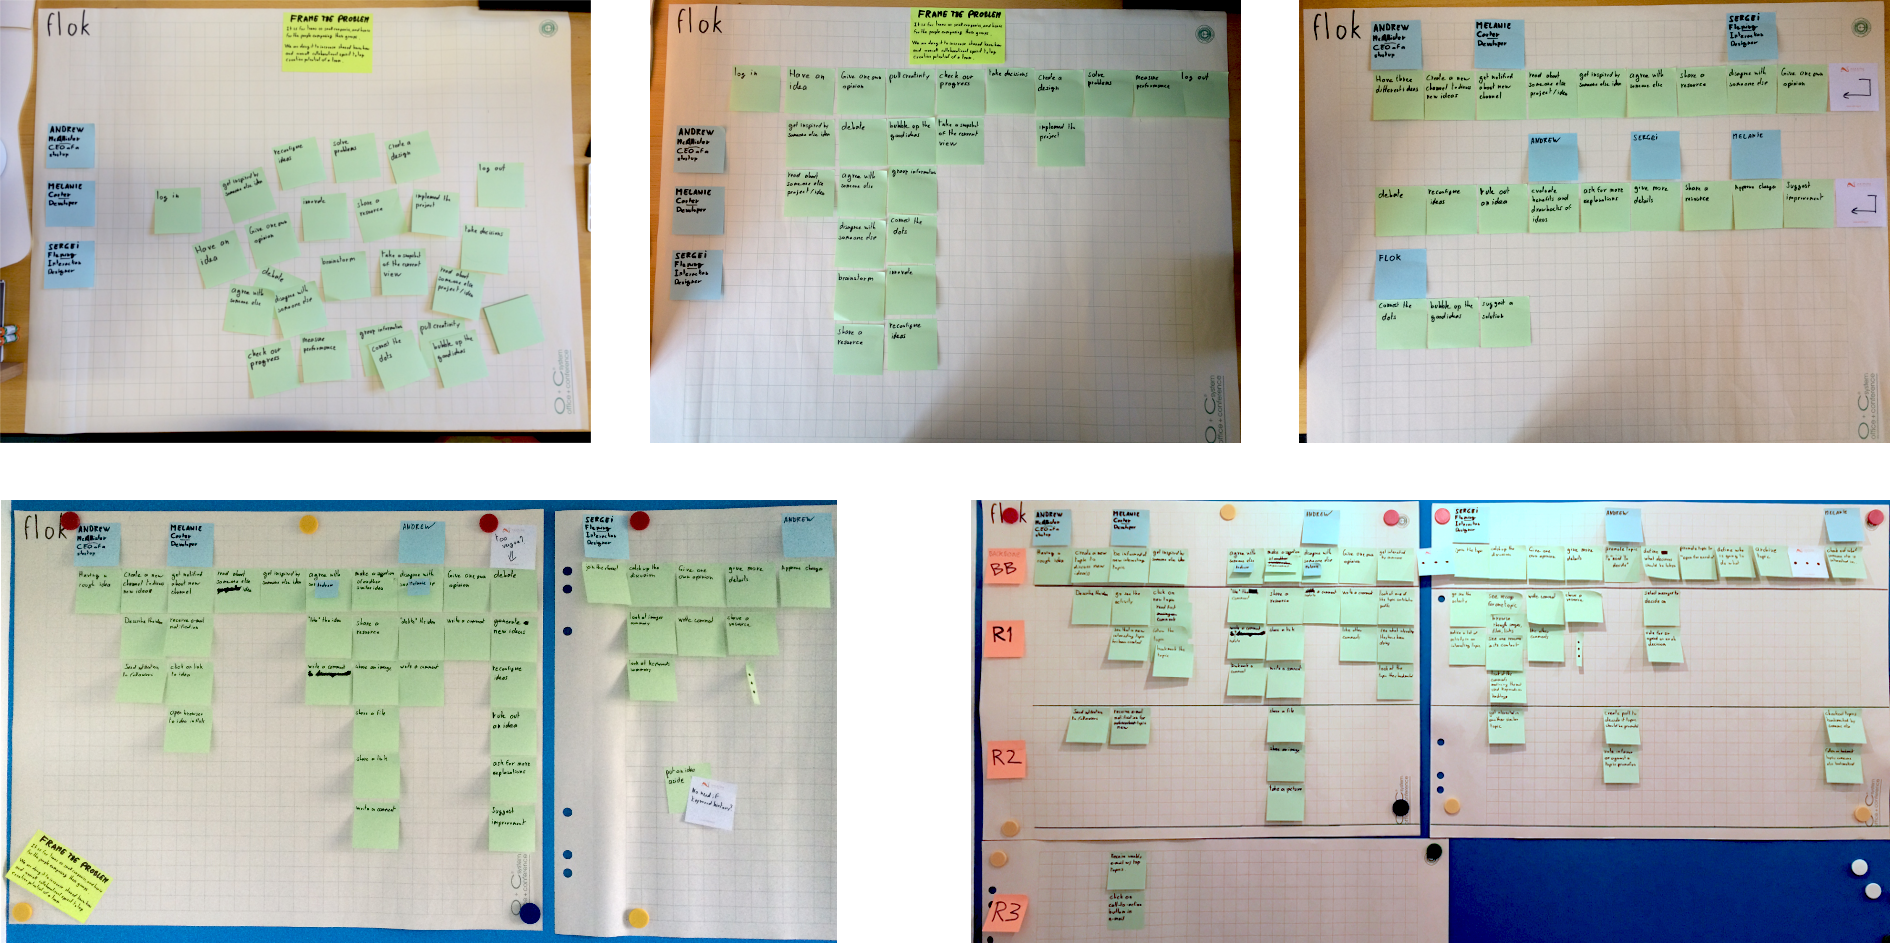
\includegraphics[width=\textwidth]{images/flokUsmEvolution.png}
\caption{Evolution of the user story map for Flok}
\label{fig.flokUsmEvolution}
\end{figure}

The user story map constantly evolves throughout the development of the project.
In figure \ref{fig.flokUsmEvolution} you have an overview of how it evolved for Flok.
Figure \ref{fig.flokUsmCurrent} shows you its state at the time of handing in this report.

% TODO Still subject to change until I hand in the report. Change the story description accordingly
\begin{figure}[!htb]
\centering
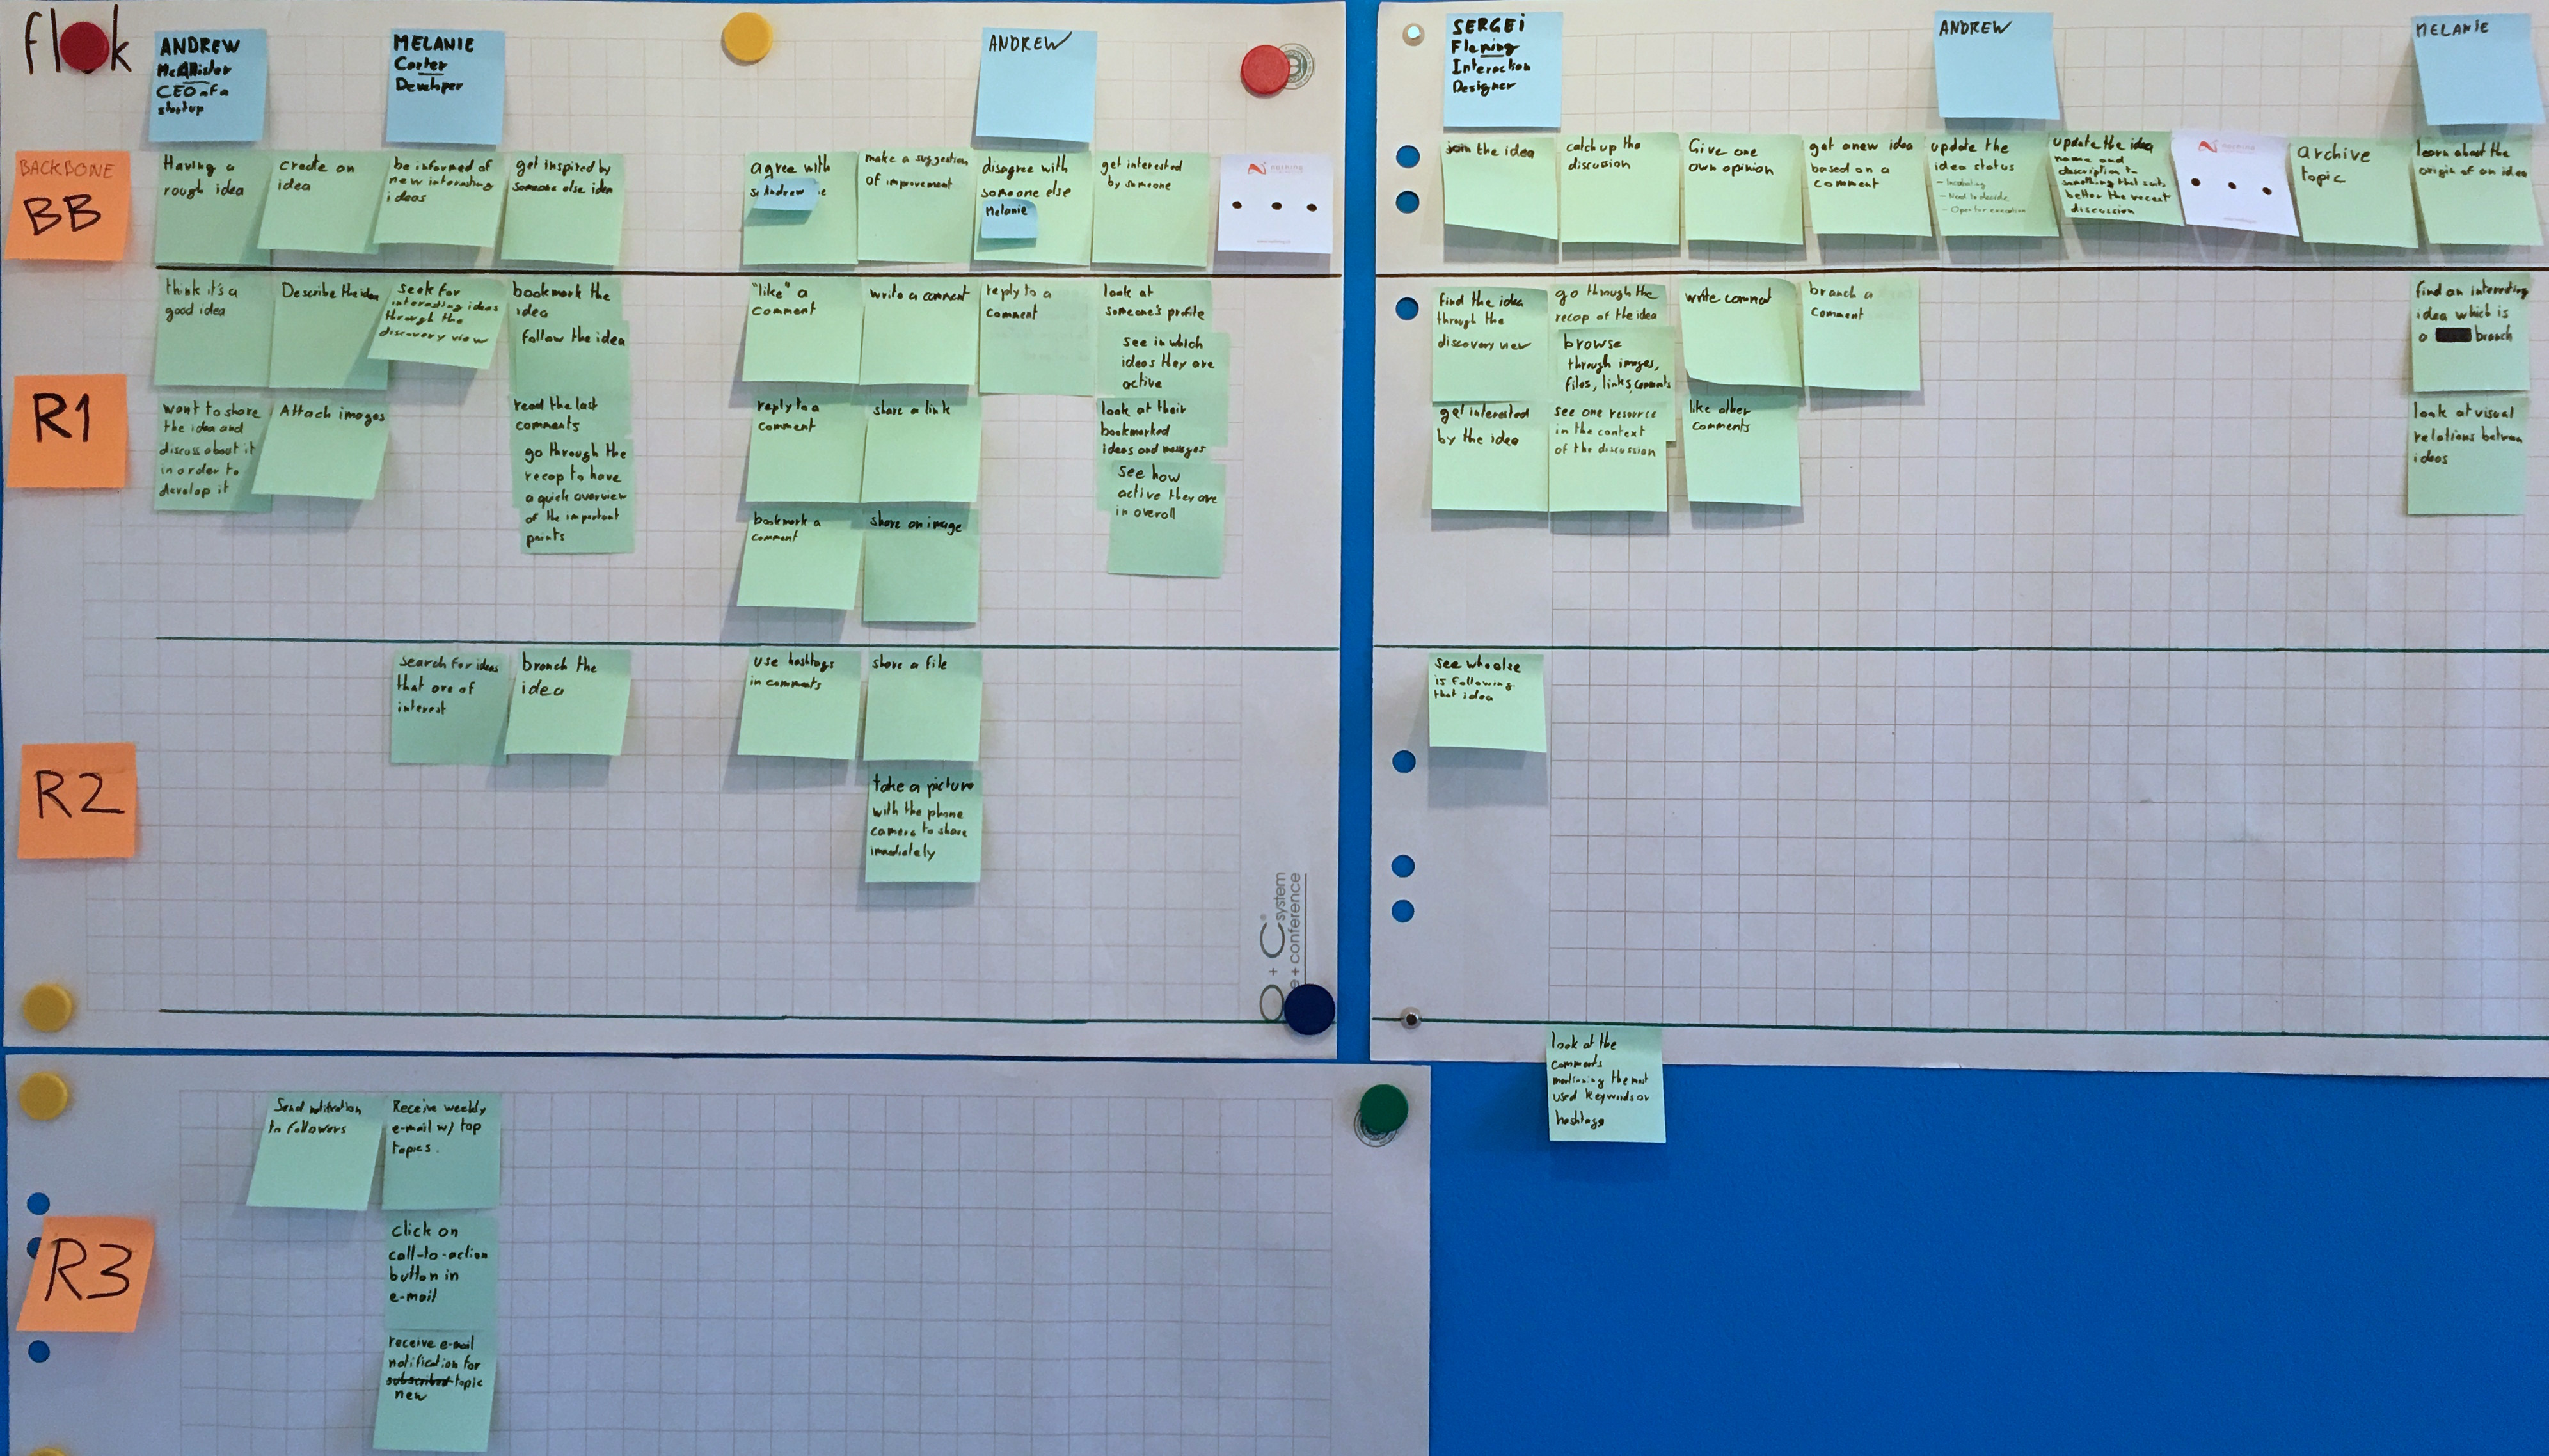
\includegraphics[width=\textwidth]{images/flokUsmCurrent.jpg}
\caption{Current state of the user story map for Flok}
\label{fig.flokUsmCurrent}
\end{figure}

The green sticky notes represent actions by users and the blue ones indicate which user are doing the actions.
In the latest versions of the user story map, we can notice that the orange sticky notes entitle \emph{slices}, of the story.
As said, the first row is the backbone.
Below we have three slices R1, R2 and R3, \emph{R} meaning \emph{release}.
It helps to define clearly which part of the story are the most important and therefore need to be possible to do for the user in the earliest versions of Flok.

Building this user story map was a bit more tricky than it can be for most others.
Indeed, as Flok interest resides in the real-time interactions between its users, the story has to jump often from a user to another.
This makes it also more difficult to follow when reading the story map.

\subsubsection*{Story description}
The story simply start with Andrew having a rough idea that he wants to share in order to discuss about it and develop it.
He then adds the idea on Flok and describe it with text, but images as well.
From here, other users can take part to the idea. For instance, Melanie is looking for interesting ideas in the \emph{discovery} section of the app and she get inspired by the one from Andrew.
From here, she has several possibilities.
She can simply bookmark the idea in order to have it saved and hence, easily come back to it later.
She can also follow the idea in order to get informed of the activity occurring within it.
Then, as she's interested, she goes through a page which recaps the discussion around the idea.
This helps her to quickly have a good overview.
If she wants to actively take part to the idea, she can go to the discussion section and read the last comments before interacting.
As it happens, she agrees with Andrew's comment and show it by \emph{liking} it and replying directly to it.
Moreover she wants to find that comment later so she bookmarks it.
Then she gives her input by writing comments and sharing documents and images.
However, Andrew disagrees with the input from Melanie and he says it by replying to the corresponding comment.

Among the comments and other inputs of team mates taking part to Andrew's idea, he gets interested by the views of one specific person.
He looks at this person profile and more precisely in which other ideas she's active and that might interest him.

Back to Andrew's idea, after a while, Sergei joins the idea that he found through the \emph{discovery} section of the app.
He found the idea interesting and noticed that among the followers there were team mates he usually like their thinking.
He catches up the discussion through the recap and among the highlighted items one image appealed him.
He brings up the image in its context to see in more details what it is about.
This makes him think about another idea so instead of replying at this point of the discussion, he rather decides to fork from the image to create a new idea in Flok.

Initially new ideas are classified under the \emph{Incubating} label.
This is not the case anymore for Andrew's idea which has evolved and became more mature and precise.
Hence he decides to update the classification to \emph{Need to decide} where the discussion should be more about what are going to be the next step to implement the idea.
Moreover, the original name and description of the idea do not suit its content anymore.
Therefore Andrew updates them accordingly.

After a while, the idea reached the \emph{Open for execution} classification where it got successfully implemented.
At this point the idea can be archived, which is what Andrew does.

% TODO link the story map to the hypothesis.

\section{Information architecture}
To accompany and solidify the project it is important to have a good information architecture.
This helps to have a well defined vocabulary for the different elements making the product, and how they interact with each other.
In our case, we made an \emph{entity-relationship diagram} that you can see in figure \ref{fig.erDiagram}.
In the rectangle are the different entities in Flok.
The ovals their attributes and the diamonds are actions representing the relation between entities.
We have to read the relations from top to bottom (e.g. \emph{Persons are actor of Activity items} or \emph{Ideas contain Messages}).
The thickness of the lines and the fact they are an arrow or not also has a specific meaning, described in the bottom right of the figure.
For instance, a person can post none or more messages, but a specific message is posted by exactly one person.
Also, a message must be either an image, a file, a system information or a comment, and any of these four entities has to be a message.

% TODO decide what to do with hashtags, keywords and links that are currently not supported in the platform
\begin{sidewaysfigure}[!ht]
\centering
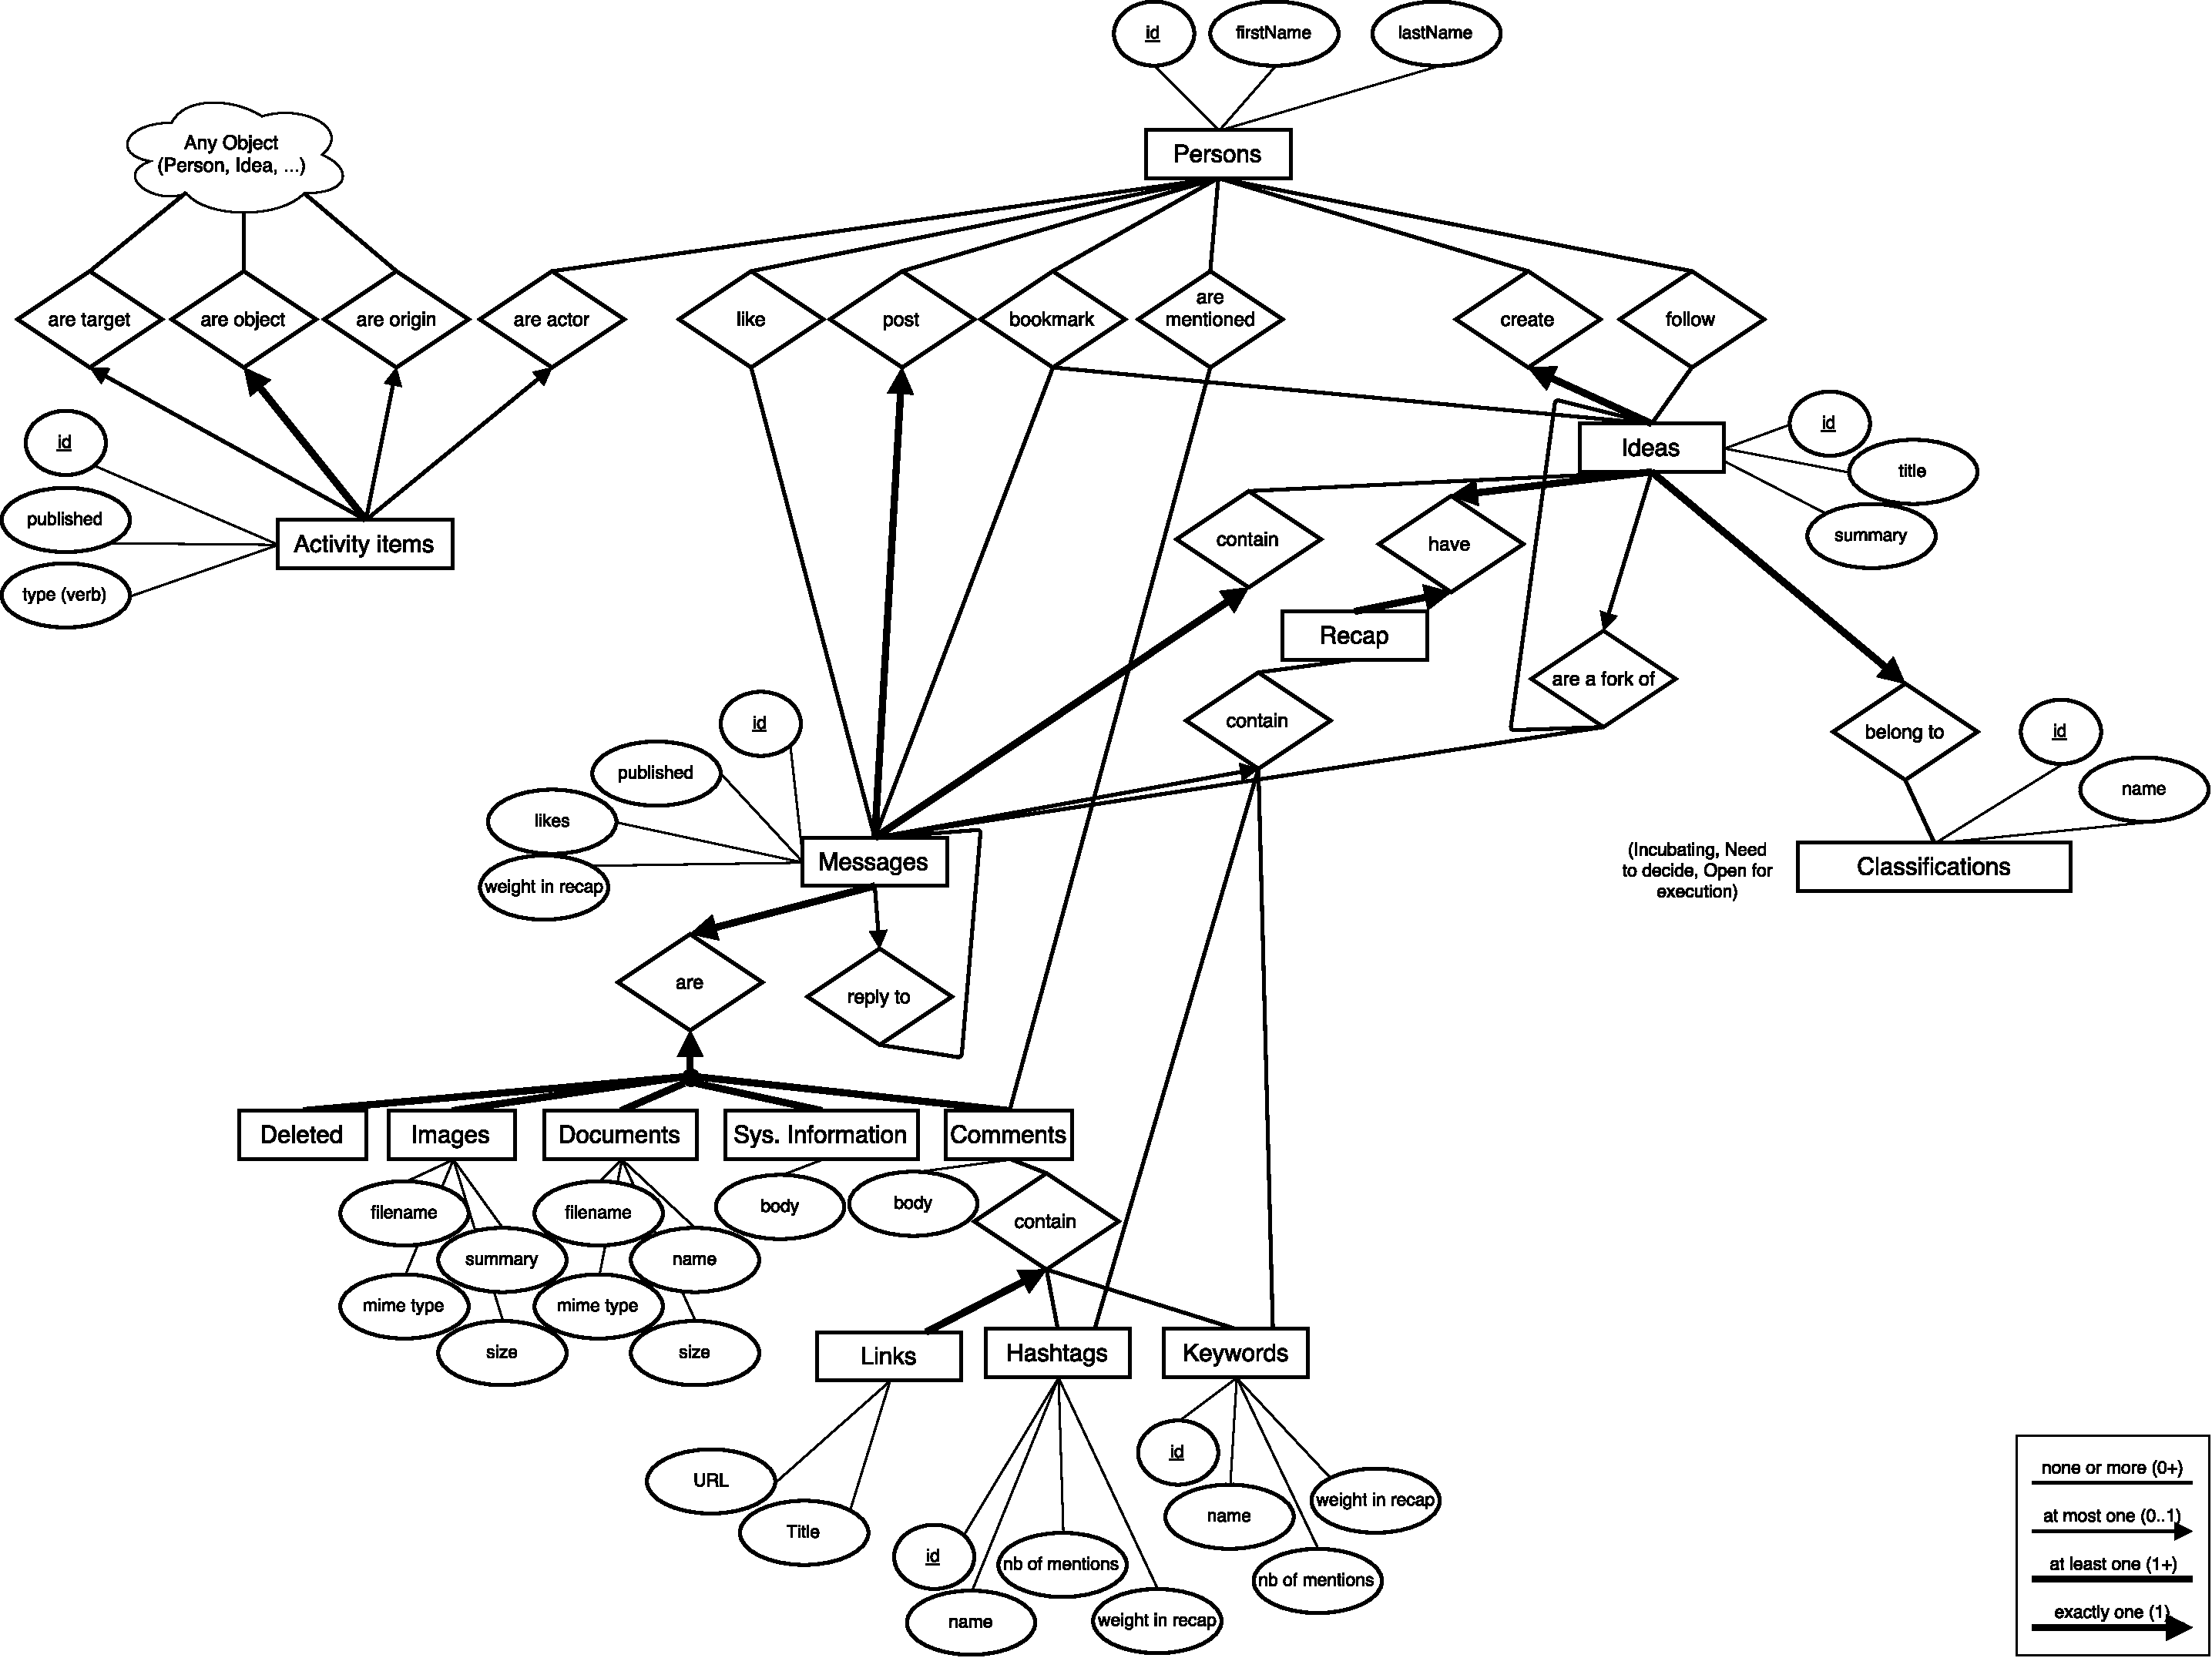
\includegraphics[width=\textwidth]{images/erDiagram.pdf}
\caption{The entity-relationship diagram of Flok, representing its information architecture}
\label{fig.erDiagram}
\end{sidewaysfigure}

\clearpage

\section{Wireframing}
Once we had a first version of the user story map, the next step was to build wireframes of the user interface.
Wireframes allow to quickly have a very rough view of the components layout and how they fit in the available space.
They enable us to see changes that need to be brought even before we start designing or implementing, and hence save us some precious time.

For instance, initially ideas were called \emph{topics} and when I designed the first wireframes of recap page for a topic, it was a kind of tag cloud with all the ideas discussed in a topic – The most discussed ones being more prominent (see figure \ref{fig.originalRecapWireframes}).
This made us realize two things.
First, there was a lack of shared understanding regarding the scope of the discussions we expect to be held in one topic and therefore also regarding the content of the recap page.
Secondly, the name \emph{topic} wasn't a good name to describe this concept.
This is what made us change the name for \emph{idea}. It is also more human – Instead of creating a topic on Flok when you have an idea, you just add an idea on Flok when you have one.
This shows that we were able avoid having to change a single line of code to apply this change as it was detected before we start the first prototype.

\begin{figure}[!htb]
\centering
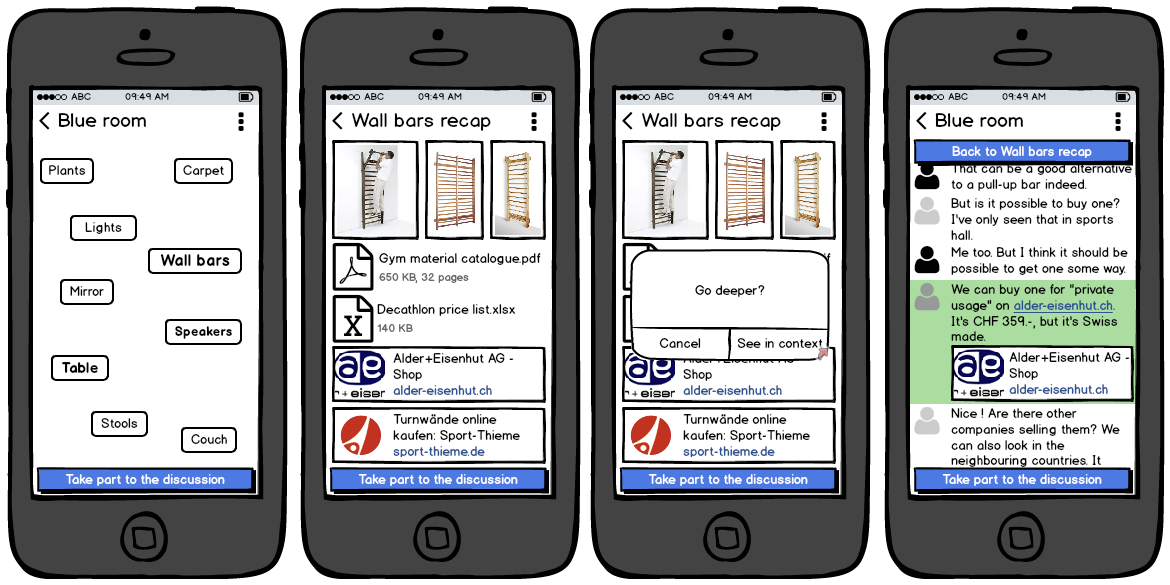
\includegraphics[width=\textwidth]{images/originalRecapWireframes.png}
\caption{Original wireframe design of the recap page. From left to right: the main recap page, the recap page of one idea in the topic, the dialog asking if we want to see an item in its context, an item highlighted in its context.}
\label{fig.originalRecapWireframes}
\end{figure}

You can notice in the wireframes of figure \ref{fig.originalRecapWireframes} that we choose to represent the app in a mobile screen.
This decision has been made because having less space forces us to think about what is the most important to show to the user.
It is then easier to design a desktop version from the mobile version than the other way around.
The \emph{Mobile First} development is also getting more important as more people are accessing the web from their mobile device before doing so from a desktop computer.

A few other design decisions were taken during wireframing.
For instance, it was initially possible to unlike a message in a discussion.
This has been removed to only keep the like button.
Indeed, it is not necessary to explicitly express a disagreement with this action which doesn't bring any constructive feedback and we also want to foster positivity.
A disagreement can still be express with a comment which should be more constructive.

This is also while designing the wireframes that we asked ourselves the question regarding the order the messages in a discussion.
Some researches \cite{mabande2010designing} concluded that having the oldest ones at the top and the more recent ones at the bottom was leading to more engagement from the participant of a discussion.
Following this order is also more human as it follows the natural reading order.
Moreover, as the input field to add messages is at the bottom, having the new messages appearing right above it is also expected.

% TODO link the wireframes to the hypothesis

\section{Prototyping}
The step following wireframing is prototyping.
In this case, the initial goal was to make it mostly visual in order to have a good idea of the look and feel, but also of the possible interactions from the users.
The content would consist of static mock data.
To avoid having to create a full visual design, we decided to use the component library \emph{Material Design Lite}\footnote{\url{http://getmdl.io}}, which is an implementation of \emph{Material Design}\footnote{\url{http://google.com/design/spec}}.
This lightweight library, with the use of some HTML, CSS and simple Javascript, enabled us to quickly have a prototype with a solid visual design (see figure \ref{fig.firstPrototypeScreenshots}).

\begin{figure}[!htb]
\centering
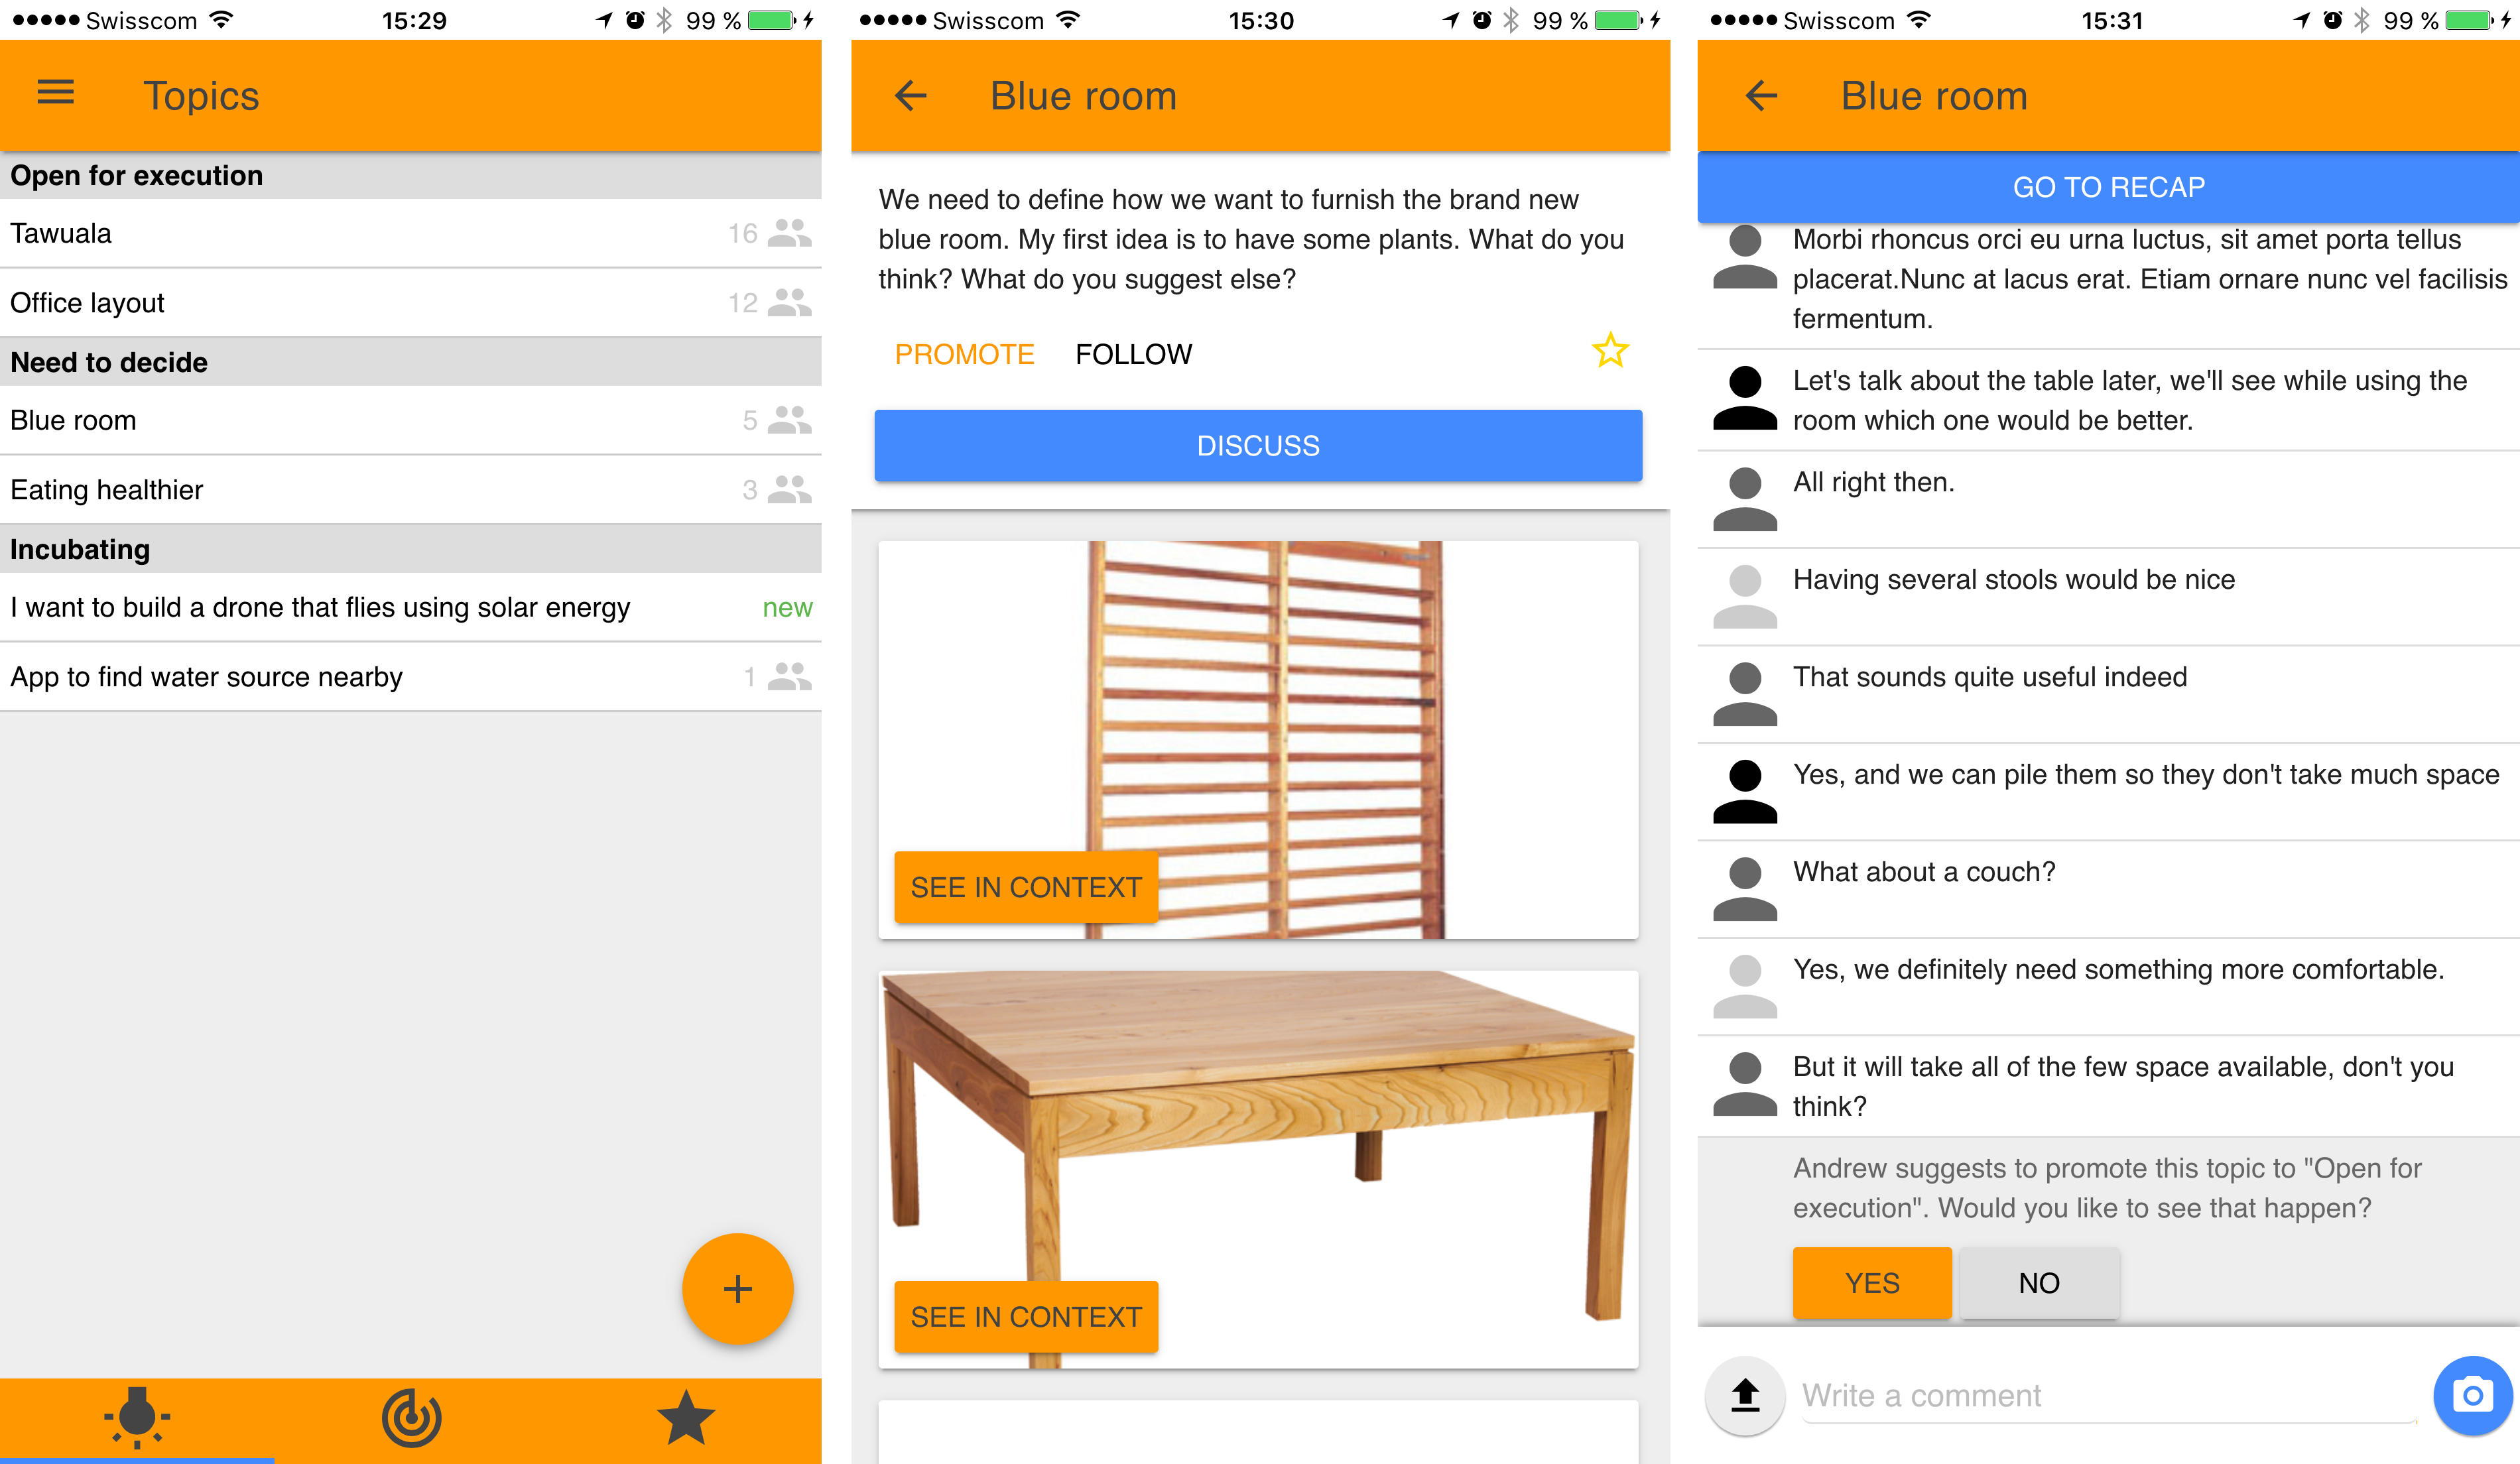
\includegraphics[width=\textwidth]{images/firstPrototypeScreenshots.png}
\caption{Screenshots of Flok first prototype using \emph{Material Design Lite}}
\label{fig.firstPrototypeScreenshots}
\end{figure}

Improvements and features have been progressively added to the prototype.
With, all the necessary code to keep it interactive.
However, as it was initially planned to be light, having a bigger code base was not adapted with the prototype structure making it quite messy and therefore more difficult to add new components.
The visual result being good, it seemed to be the right moment to start working on the functional front-end of the platform, based on the prototype.

\section{Front-end}
\subsection{Architecture}
We wanted the platform to be fully usable from any device.
The easiest way to implement that is to have a responsive web application.
Hence, Javascript and the \emph{MEAN stack} seemed quite appropriate.
These are also technologies in which \emph{Nothing Interactive} has good experience with.
This means that regarding the front-end we went for a single page application made with \emph{AngularJS}.

As we were satisfied with the result of using \emph{Material Design} for the prototype, we wanted to continue following those guidelines.
Obviously, \emph{Material Design Lite} was not enough, therefore we had to use another implementation.
Looking at the different alternatives and knowing that we were going to use \emph{AngularJS}, the decision to use \emph{Angular Material}\footnote{\url{https://material.angularjs.org}} was straightforward.

There are different ways to build an \emph{AngularJS} application.
Therefore it was important that we clearly define how we were going to structure it.
\emph{Nothing Interactive} has some internal guidelines, but with the arrival of \emph{Angular 2}, it seemed to be a good time to re-think those guidelines in order to write code that would enable an easy transition to this disruptive new version of the framework.
Hence, we made some adaptations based an Angular Style Guide written by John Papa\footnote{\url{https://github.com/johnpapa/angular-styleguide}}, which is endorsed by the Angular team.

% TODO: give detail on the app internal structure? Schema of relationship between services, directives, controllers, templates, models

Unfortunately, our great focus on building the front-end and having the best user experience possible didn't gave us time to build a functional back-end for the app.
At some point we had to take the decision between either building the back-end, or doing the user testing.
The latter seemed more important as it would (in)validate our assumptions regarding the interaction of the user with the platform.
We also estimated that it would bring us valuable feedback to improve the front-end.

Not having a back-end implies some restrictions.
First, it means that once the Angular app is loaded in the browser, everything is happening in the browser only and there is no communication with the server, except to get static files such as images.
Therefore, interaction between two users is not possible.
Then, no back-end means no database and no saved data.
Fortunately, as the front-end is a single page application, as long as the page is not fully refreshed, all the data created by the user while using Flok is saved in memory, including uploaded files.
Therefore the user can still use and evolve in the app.

We were not trying to build a fully working application without backend.
Therefore we still kept in mind an architecture that would communicate with a back-end by simulating calls to it, even though we just get the data from memory.

\subsection{Implementation}
% Recap, Classification, Activity, Messages, ...

\subsection{Design decisions}

\section{User testing}

\section{Conclusion}

\clearpage
\bibliographystyle{ieeetr}
\bibliography{main}

\end{document}
